\section{Converged Graph Relational Optimizer}

\subsection{Overview of the Framework}

A system overview figure and some introduction


\subsection{Leveraging Benefits of Both Relational and Graph Optimizations}

\begin{figure*}
    \centering
    \begin{subfigure}[b]{0.4\linewidth}
        \centering
        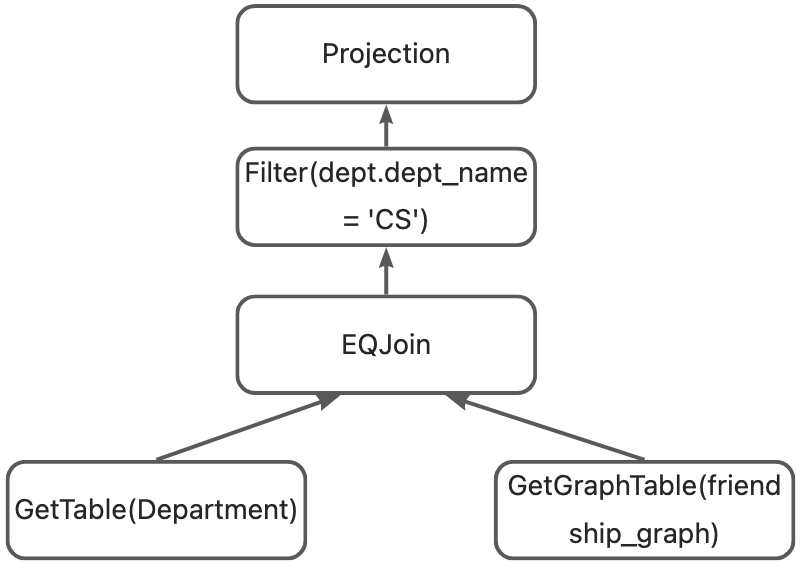
\includegraphics[width=\linewidth]{./figures/converged-logical-plan-relational.png}
        \caption{Relational Subplan of the Converged Logical Plan.}
        \label{fig:converged-logical-plan-relational}
    \end{subfigure}
    \begin{subfigure}[b]{0.4\linewidth}
        \centering
        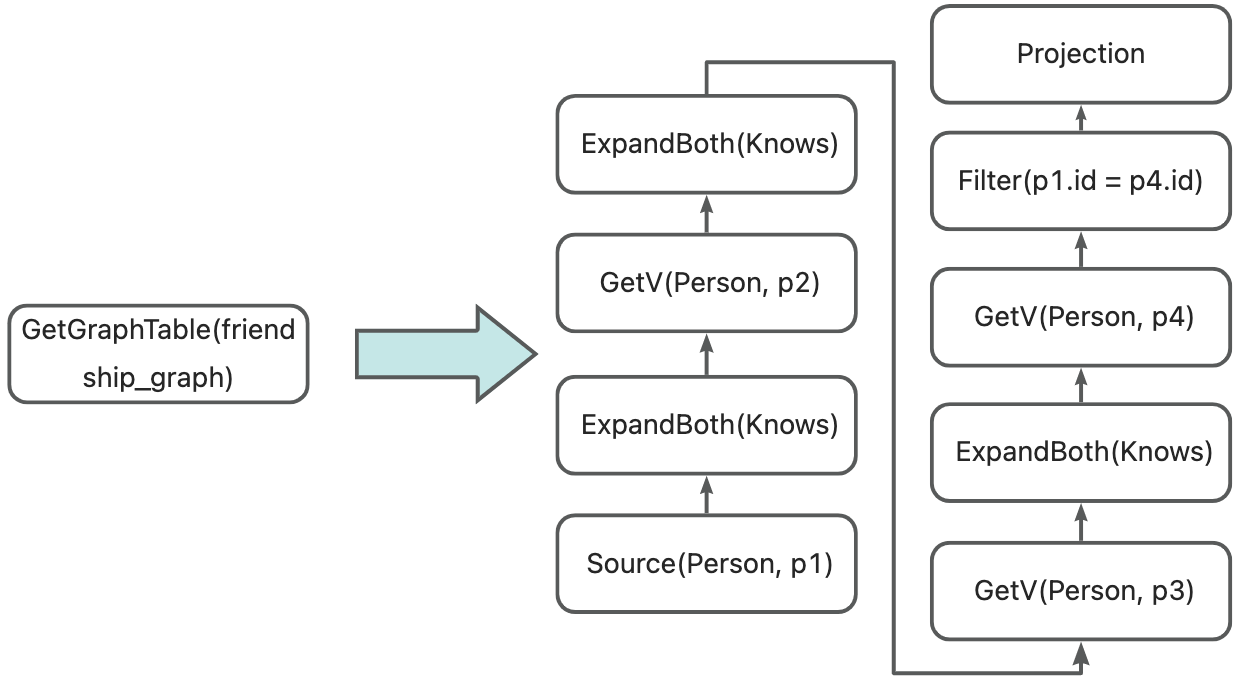
\includegraphics[width=\linewidth]{./figures/converged-logical-plan-graph.png}
        \caption{Graph Subplan of the Converged Logical Plan.}
        \label{fig:converged-logical-plan-graph}
    \end{subfigure}
    \begin{subfigure}[b]{0.4\linewidth}
        \centering
        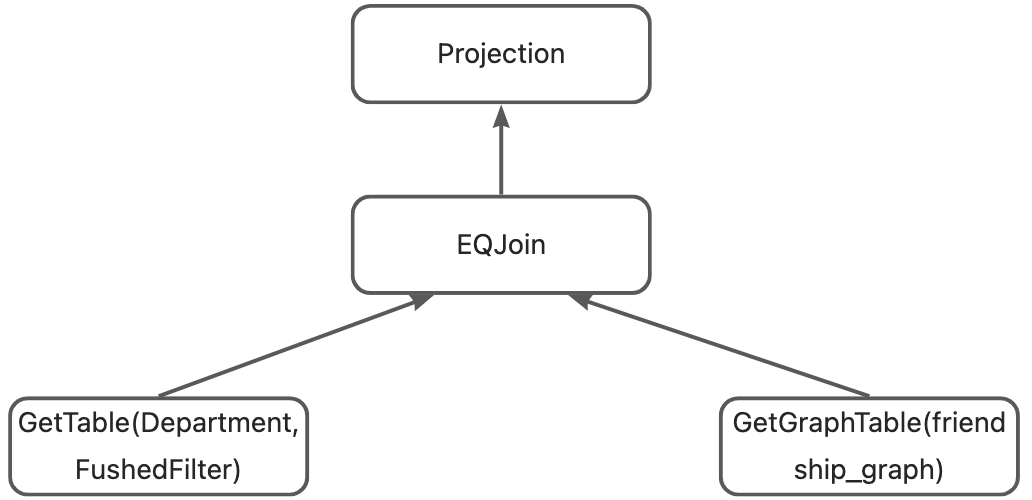
\includegraphics[width=\linewidth]{./figures/converged-logical-plan-relational-optimized.png}
        \caption{Relational Subplan after Optimization.}
        \label{fig:relational-plan-optimized}
    \end{subfigure}
    \begin{subfigure}[b]{0.4\linewidth}
        \centering
        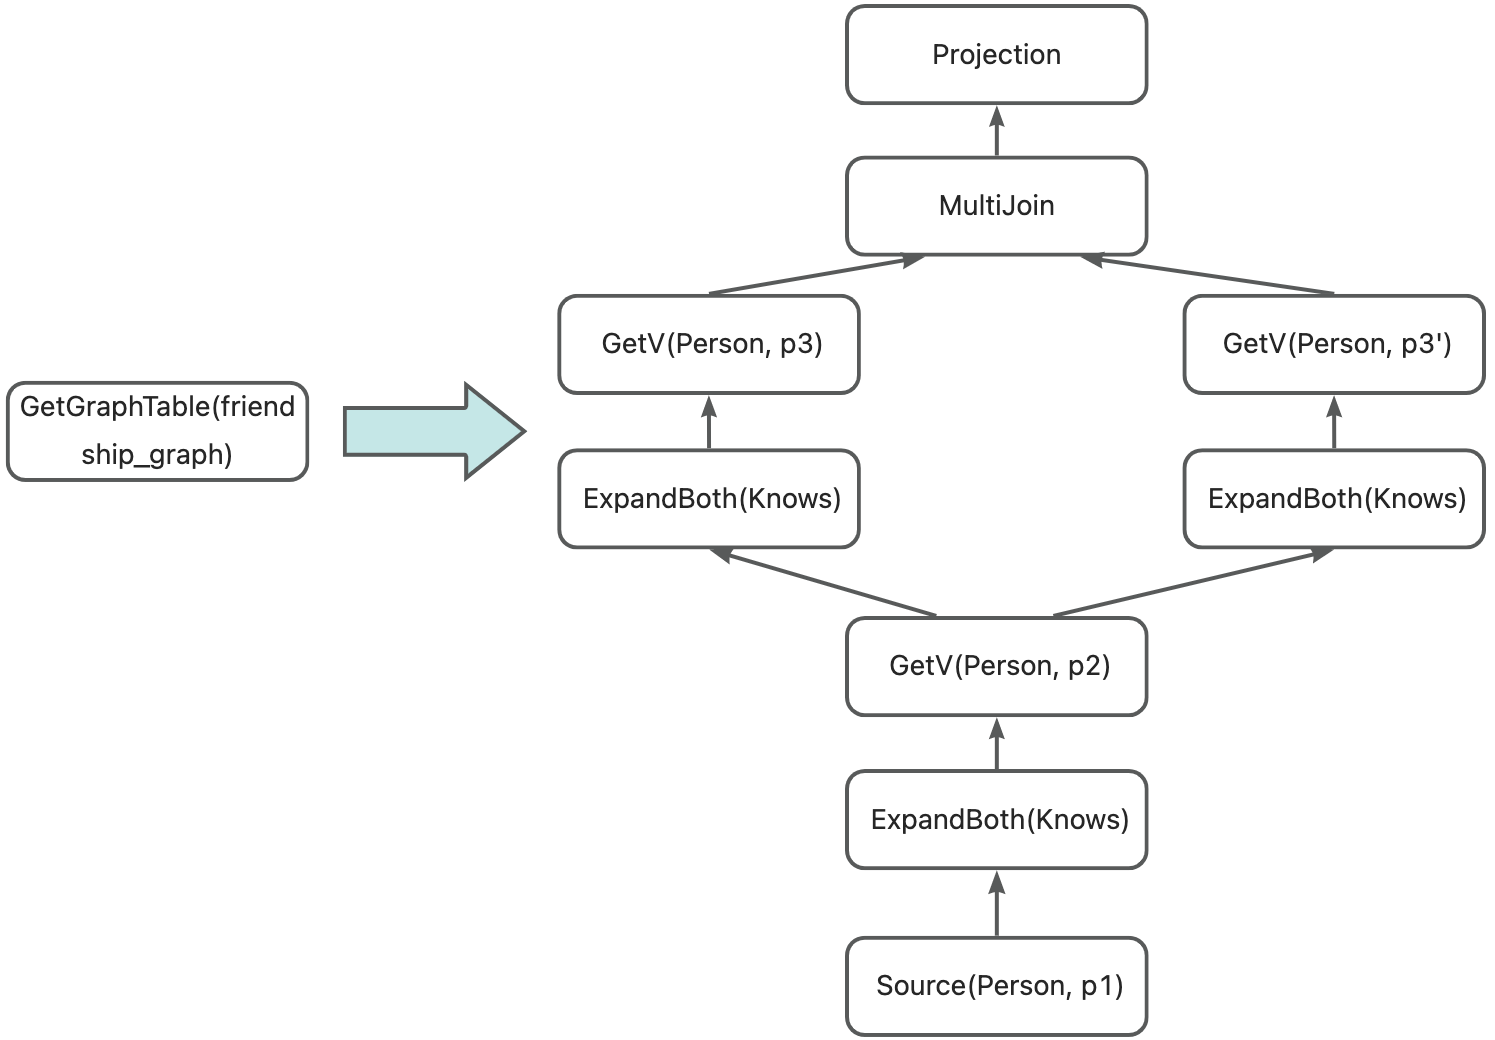
\includegraphics[width=\linewidth]{./figures/converged-logical-plan-graph-optimized.png}
        \caption{Graph Subplan after Optimization.}
        \label{fig:graph-plan-optimized}
    \end{subfigure}
    \begin{subfigure}[b]{0.4\linewidth}
        \centering
        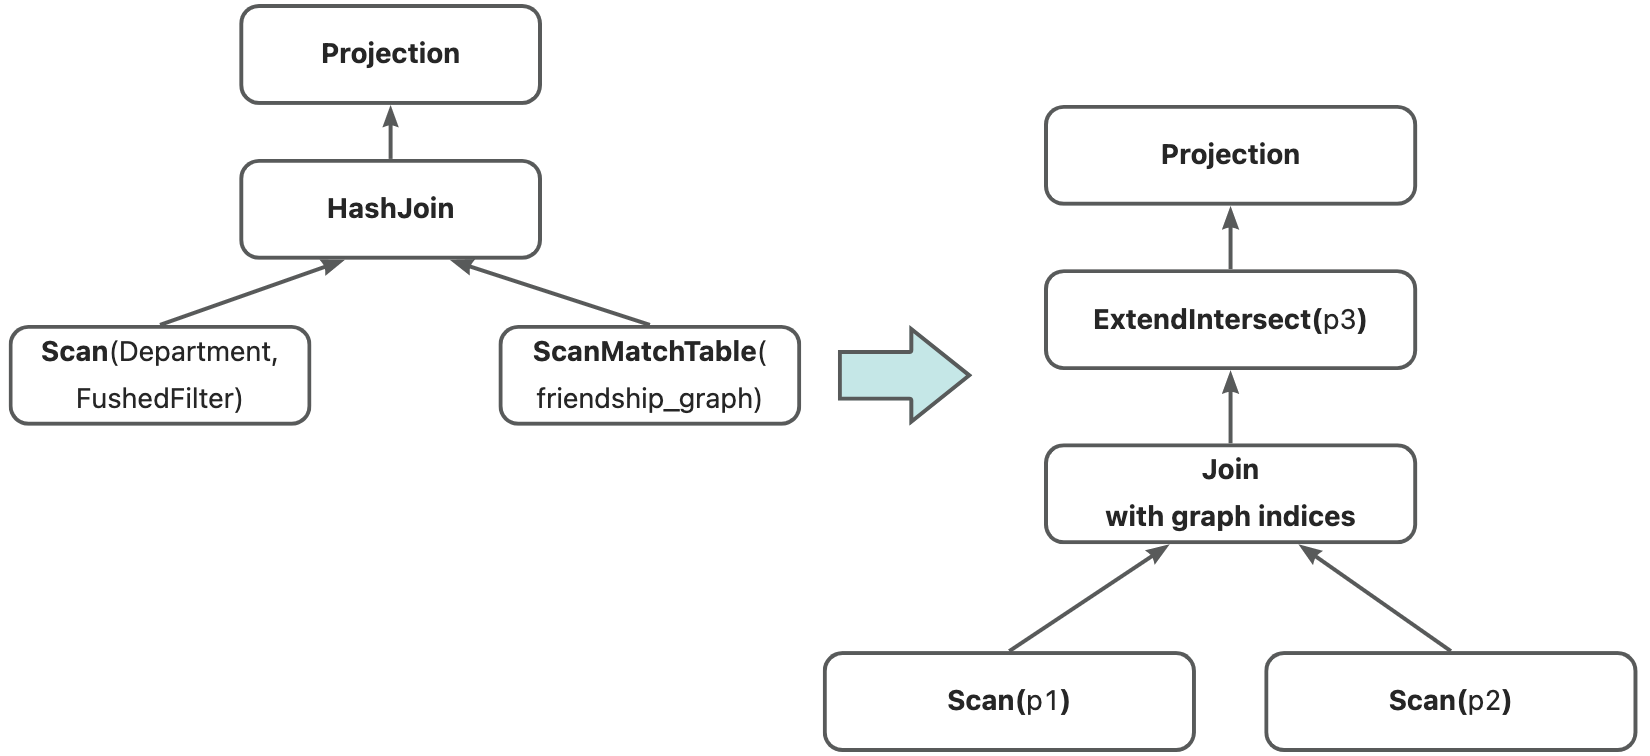
\includegraphics[width=\linewidth]{./figures/converged-physical-plan.png}
        \caption{Obtained Optimial Physical Plan.}
        \label{fig:physical-plan-optimized}
    \end{subfigure}
    \caption{An example of query opitmization.}
    \label{fig:query-grtree-example}
\end{figure*}


Given a query that follows the grammar of SQL/PGQ, it is first parsed and a converged logical plan is generated.
The converged logical plan consists of several graph subplans and a relational subplan.
Eacn graph subplan corresponds to a graph query, and it is optimized with graph optimizers.
Since parts of the graph query are always marked with ``GRAPH\_TABLE (name, MATCH $\cdots$)'', it is straightforward to distinguish graph queries from relational queries, and the graph subplans can be generated easily.
For each graph subplan, an operator ``GetGraphTable(name)'' is generated and added to the relational subplan.
Specifically, from the perspective of relational optimizers, the ``GetGraphTable'' operator is simply an operator for retrieving data like ``GetTable'' and it returns table data.
Please note that in a SQL/PGQ query, a graph query can be utilized as a subquery to retrieve the table involved in the relational query.
However, a relational query cannot serve as a subquery within a graph query because the mapping between tables and vertices/edges need to be specified beforehand.


With the generated converged logical plan, the converged optimizer takes effect and obtains the optimal physical plan by applying different optimization strategies.
The strategies are of two types, i.e., rule-based optimizations (abbr.~RBO) and cost-based optimizations (abbr.~CBO).
In our converged graph relational optimizer, strategies for relational queries and graph queries are utilized for the relational subplan and graph subplans, respectively.
Moreover, there are also some optimization strategies that intersect and interact throughout the graph and relational query optimization processes.
These strategies will be detailed in Section \ref{sec:detailed-optimizations}.

After the optimal physical plan is obtained, it is fed to the executor to get the query results.
Although different databases can have different operators and different requirements for physical plans, the physical plan for one database can be converted to that for another database by exploiting Codegen.
Specifically, the original physical plan is firstly converted to an internal representation (e.g., substrait), and then the internal representation is transformed to the physical plan of the target database.
The above process of query processing is illustrated with the following example.

\begin{example}
    Given a relational database with tables as follows,
    \begin{equation*}
        \begin{split}
            & \textit{Person = (\underline{id}, name, dept\_id)} \\
            & \textit{Knows = (\underline{id1}, \underline{id2})} \\
            & \textit{Department = (\underline{dept\_id}, dept\_name)}, \\
        \end{split}
    \end{equation*}
    suppose we are going to find three persons satisfying: 
    (1) These three persons know each other;
    (2) At least two of them are from the department of computer science.
    The SQL/PGQ query for this task is shown in Example \ref{example:introduction:sqlpgq}.      

    There is one graph query for obtaining triangles of persons that know each other.
    Therefore, the converged logical plan consists of one relational subplan and one graph subplan.
    The algebra expression corresponding to this query is as follows:
    Firstly, to obtain the triangles, the graph relational algebra expression is
    \begin{equation*}
        \begin{split}
            G_{\triangle} = & \sigma_{p4.id = p1.id}(\updownarrow_{(p3)}^{(p4)}[:Knows]\updownarrow_{(p2)}^{(p3:Person)}[:Knows] \\
            & \updownarrow_{(p1)}^{(p2:Person)}[:Knows]\bigcirc_{(p1:Person)}).
        \end{split}
    \end{equation*}
    Then, to get the results of the graph query and formulate the results as a relational table, the algebra expression is 
    \begin{equation*}
        \begin{split}
            R_{graph} = & \pi_{p1.name\rightarrow pn1, p1.dept\_id \rightarrow dept1,p2.name\rightarrow pn2, p2.dept\_id \rightarrow dept2,} \\
            & _{p3.name\rightarrow pn3, p3.dept\_id \rightarrow dept3}(G_{\triangle}).
        \end{split}
    \end{equation*}
    Finally, to obtain the triangles of persons with at least two persons from the department of computer science, the relational algebra expression is
    \begin{equation*}
        \begin{split}
        \pi_{pn1, pn2, pn3}
        (& \sigma_{dept.dept\_name = `Computer Science'}( \\ 
        & dept \Join_{dept1=dept.dept\_id \land dept2=dept.dept\_id} R_{graph})).
        \end{split}
    \end{equation*}

    Based on the above algebra expressions, the corresponding converged logical plan is shown, and its relational and graph subplans are presented in Fig.~\ref{fig:converged-logical-plan-relational} and Fig.~\ref{fig:converged-logical-plan-graph}, repsectively.
    
    Then, optimization strategies are applied to optimize the relational subplan and graph subplans.
    The optimized converged logical plan is shown in Fig.~\ref{fig:relational-plan-optimized} and Fig.~\ref{fig:graph-plan-optimized}.
    Moreover, the finally obtained optimal physical plan is shown in Fig.~\ref{fig:physical-plan-optimized}.
\end{example}

\subsection{Detailed Optimizations}
\label{sec:detailed-optimizations}

In this subsection, we first present the optimization strategies for the relational subplan and graph subplans, respectively.
Then, the strategy interacts relational subplan and graph subplans are proposed.

\subsubsection{Optimization Strategies for Relational Subplans}

Like most relational optimizers, we have applied both Rule-based Optimization (abbr.~RBO) and Cost-based Optimization (abbr.~CBO) strategies on relational subplans for a better physical plan.
In detail, in terms of RBO, commonly used optimizations such as filter pushdown, join order optimization, and removal of unused columns are employed in the converged optimizer.
In terms of CBO, the costs of plans are estimated based on the low-order statistics such as the cardinality of tables and query conditions.



\subsubsection{Optimization Strategies for Graph Subplans}

We have formulated a specific rule set to capitalize on optimization potential among graph operators. 
Both RBO and CBO strategies are included in the rule set.

In terms of RBO strategies, two frequently utilized key rules, i.e., \trimrule and \fusionrule, are presented in this subsection.

\trimrule. 
The \trimrule~ is a well-established relational optimization strategy that removes superfluous data at intermediary stages of query processing. 
Two particular instances where trimming helps include: 
Firstly, \trimrule~ can eliminate intermediate results with aliases that are not required and reduce computations.
Secondly, it involves discarding unneeded vertex and edge properties when retrieving from the data graph. 
This is accomplished by specifying essential properties in the graph operators’ \code{COLUMNS} field.

\fusionrule. 
The \fusionrule~ is a graph-centric rule. 
Commonly in graph queries, a sequence of \expandedge~ followed by \getvertex~ indicates a search for neighboring vertices. 
The \fusionrule~ consolidates these operators into one integrated \expandvertex~ to boost efficiency. 
Nonetheless, whether \expandedge~ and \getvertex~ can be merged is context-dependent. 
For example, if some properties of the edges are needed, fusion might not be feasible.
This rule evaluates such factors to ensure query optimization without compromising result integrity.


In terms of CBO, drawing from insignts gained in the prior research, we implement effective pattern matching by incorporating hybrid pattern join strategies and leveraging high-order statistics, which provide a more granular understanding of the data through the frequency of smaller patterns.
Moreover, the prior research has some drawbacks, including using a bottom-up search framework that potentially missed early pruning opportunities and having a narrow focus on basic patterns without accommodating union patterns scenarios.
Therefore, we also introduce a novel top-down search framework, inclusive of branch-and-bound pruning strategies, and devise specific cardinality estimation methods for union patterns. 
Besides, in this implementation, we use a rule for pattern transformation to ensure all modifications maintain the original results’ integrity.
Furthermore, for pattern matching, we consider binary join and extend-intersect operators. 
The binary join applies a hash-join on two pattern mappings to produce a larger pattern's results.
The extend-intersect operator optimizes the process when only one vertex is added to the existing pattern. 
This expansion can vary from a simple addition of a single new edge to more complex scenarios involving multiple edges, implemented through optimal joins.

Regarding cost and cardinality estimation, we adopt a cost model that considers both the communication costs of intermediate result transfer in distributed environments and the computational costs of physical plan operators. 
Specifically, costs for the binary join and extend-intersect operators in graphs are defined. 
Additionally, we estimate the operator cost using an expand ratio that reflects the change in pattern occurrences when edges are expanded.

\subsubsection{Interacting Strategies}

Please note that the optimization of graph subplans and the relational subplan are not isolated or entirely unconnected.
For example, when \trimrule~ is applied on graph subplans, it is necessary to judge whether the properties of vertices and edges are utilized in graph subplans and relational subplans.
Besides, more interacting optimization strategies can be designed for optimizing the graph and relational subplans simultaneously.
One crucial strategy among the possible ones is \filterrule. 

\filterrule. 
The \filterrule demonstrates a graph-relational optimization that highlights the synergy between graph and relational optimization. 
Given a SQL/PGQ query, the constraints on a graph element can be specified in the relational or graph parts.
For instance, 
\begin{lstlisting}
    F1:
        SELECT p FROM GRAPH_TABLE (friendship_graph 
        MATCH (p1:Person)-[:Knows]-(p2:Person {name = 'John'})
        COLUMNS (p1.name as p));
\end{lstlisting}
and 
\begin{lstlisting}
    F2:
        SELECT p FROM GRAPH_TABLE (friendship_graph 
        MATCH (p1:Person)-[:Knows]-(p2:Person)
        COLUMNS (p1.name as p, p2.name as p2))
        WHERE p2 = 'John';
\end{lstlisting}
both find persons that know John.
Their only difference is that F1 specifies the constraints in the graph query, while F2 specifies the constraints in the relational query.
It is obvious that F1 is more efficient since persons whose names are not John cannot match p2 in the graph query and the graph query returns fewer results.
Therefore, it is necessary to push down filtering conditions in SQL/PGQ queries.
Specifically, the \filterrule aims to introduce such filters at the pattern matching phase. 
It seeks to push filtering conditions on properties of graph elements from the relaitonal subplan to graph subplans.
Moreover, \filterrule attemps to embed filtering conditions into basic graph operators like \scan~, \expandedge~, or \getvertex to further push down filtering conditions in graph queries. 
This integration allows the direct exclusion of vertices and edges not satisfying the filter conditions, thus drastically cutting down the volume of intermediary outcomes.
